%%%%%%%%%%%%%%%%%%%%%%%%%%%%%%%%%%%%%%%%%
% Journal Article
% LaTeX Template
% Version 1.3 (9/9/13)
%
% This template has been downloaded from:
% http://www.LaTeXTemplates.com
%
% Original author:
% Frits Wenneker (http://www.howtotex.com)
%
% License:
% CC BY-NC-SA 3.0 (http://creativecommons.org/licenses/by-nc-sa/3.0/)
%
%%%%%%%%%%%%%%%%%%%%%%%%%%%%%%%%%%%%%%%%%
%----------------------------------------------------------------------------------------
%    PACKAGES AND OTHER DOCUMENT CONFIGURATIONS
%----------------------------------------------------------------------------------------
\documentclass{article}
\usepackage[francais]{babel} % English language/hyphenation
\usepackage{amsmath,amsfonts,amsthm} % Math packages
\usepackage[utf8]{inputenc}
\usepackage{float}
\usepackage{amsmath}
\usepackage{mathtools}
\usepackage{blindtext}
\usepackage{graphicx} 
\usepackage{caption}
\usepackage[justification=centering]{caption} %centered caption
\usepackage{subcaption}
\usepackage{slashbox}
\usepackage{pict2e}
\usepackage{diagbox}
\usepackage[sc]{mathpazo} % Use the Palatino font
\usepackage[T1]{fontenc} % Use 8-bit encoding that has 256 glyphs
\linespread{1.05} % Line spacing - Palatino needs more space between lines
\usepackage{listings} % insert code

\usepackage{microtype} % Slightly tweak font spacing for aesthetics
\usepackage[hmarginratio=1:1,top=32mm,columnsep=20pt]{geometry} % Document margins
%\usepackage{multicol} % Used for the two-column layout of the document
%\usepackage[hang, small,labelfont=bf,up,textfont=it,up]{caption} % Custom captions under/above floats in tables or figures
%\usepackage{booktabs} % Horizontal rules in tables
\usepackage{float} % Required for tables and figures in the multi-column environment - they need to be placed in specific locations with the [H] (e.g. \begin{table}[H])
\usepackage{hyperref} % For hyperlinks in the PDF
\usepackage{lettrine} % The lettrine is the first enlarged letter at the beginning of the text
\usepackage{paralist} % Used for the compactitem environment which makes bullet points with less space between them
\usepackage{abstract} % Allows abstract customization
\renewcommand{\abstractnamefont}{\normalfont\bfseries} % Set the "Abstract" text to bold
\renewcommand{\abstracttextfont}{\normalfont\small\itshape} % Set the abstract itself to small italic text
\usepackage{titlesec} % Allows customization of titles

%\renewcommand\thesection{\Roman{section}} % Roman numerals for the sections
%\renewcommand\thesubsection{\Roman{subsection}} % Roman numerals for subsections

%\titleformat{\section}[block]{\large\scshape}{\thesection.}{1em}{} % Change the look of the section titles
%\titleformat{\subsection}[block]{\large}{\thesubsection.}{1em}{} % Change the look of the section titles

%\usepackage{pageno}
\usepackage{graphics}% resize tabular
\newcommand\scalemath[2]{\scalebox{#1}{\mbox{\ensuremath{\displaystyle #2}}}} %resize matrix
\usepackage{adjustbox}% resize code lstlisting

\usepackage{fancyhdr} % Headers and footers
\pagestyle{fancy} % All pages have headers and footers
\fancyhead{} % Blank out the default header
\fancyfoot[C]{\thepage} % Blank out the default footer

\fancyhead[C]{Université de Technologie de Compiègne $\bullet$ SY09 $\bullet$ P17} % Custom header text

%----------------------------------------------------------------------------------------
%    TITLE SECTION
%----------------------------------------------------------------------------------------
\title{\vspace{-15mm}\fontsize{24pt}{10pt}\selectfont\textbf{Classification automatique}} % Article title
\author{
\large
{\textsc{Yanqing ZENG~ GI05}}\\
{\textsc{Minh Tri LÊ GI02}}
}


%----------------------------------------------------------------------------------------
\begin{document}
\maketitle % Insert title
\thispagestyle{fancy} % All pages have headers and footers


\section*{Introduction}
L'objectif de ce TP est d'appliquer des méthodes de visualisation et de classification automatique afin d'explorer des jeux de données selon les similarités ou dissimilarités des individus.\\
Nous utiliserons l'ACP et l'AFTD (CMDS : Classical MultiDimentional Scaling) pour la visualisation ainsi que la classification hiérarchique et la méthode des centres mobiles (K-Means) pour la classification automatique.


\section{Visualisation des données}

Le but de cette partie est de visualiser les données dans un espace de dimension 2 avec l'ACP ou l'AFTD.

\subsection*{1.}

Les données Iris sont des mesures de certaines espèces de fleurs (3 espèces).

On effectue donc l'ACP sur ce jeu de données, d'abord sans et avec coloration pour distinguer les espèces. (Figure [\ref{iris_acp}]).
\begin{figure}[H]
\centering
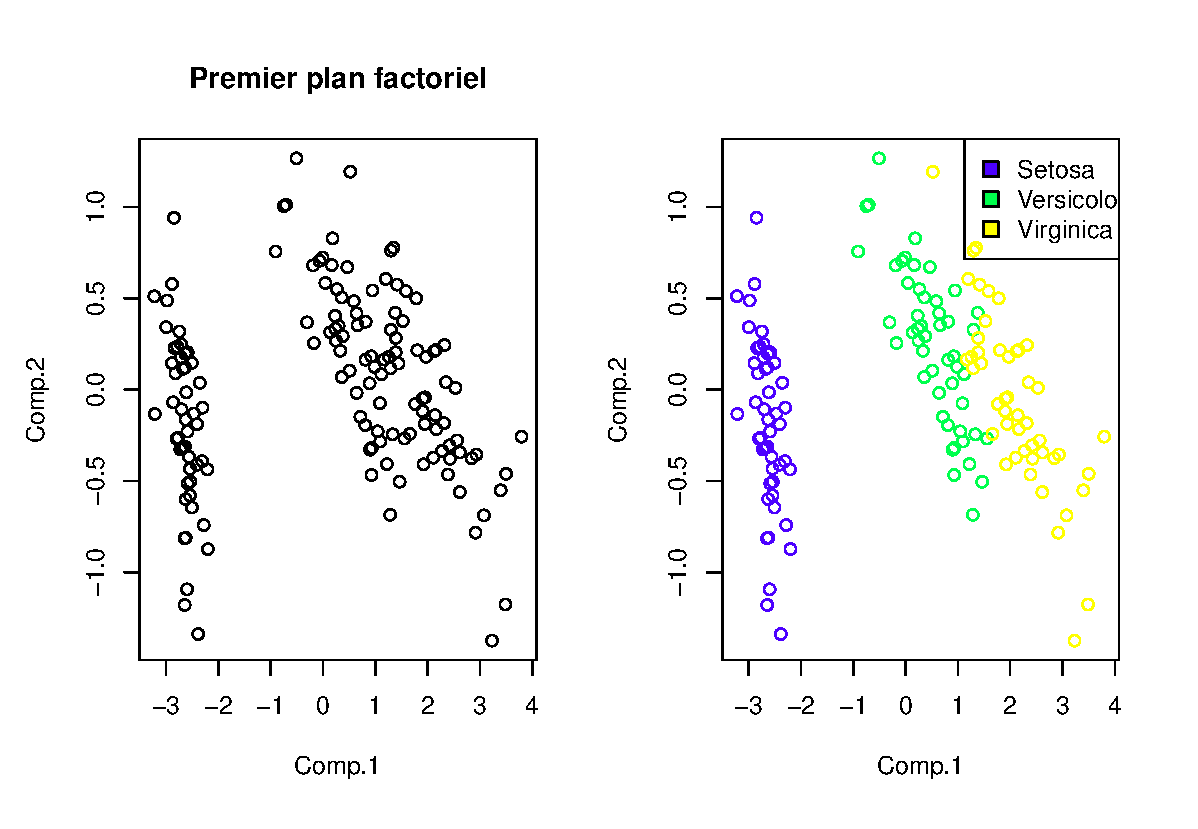
\includegraphics[scale=0.5]{./img/iris_acp.eps}
\caption{Représentation des données \textit{iris} par ACP}
\label{iris_acp}
\end{figure}

Après l'ACP, on peut facilement distinguer deux groupes sur la figure de gauche (\ref{iris_acp}).\\
Seulement, on se rend compte que la figure de droite (\ref{iris_acp}) montre en fait trois groupes. Le groupe de données de droite est en effet plus difficilement distinguable en deux groupes. Les espèces Versicolor et Virginica sont assez proches.

Il en résulte que si l'on recherche une partition de donnée et si le nombre K de partitions vaut 2, les Versicolor et Virginica seront dans le même groupe. Avec K=3, les partitions correspondront aux trois espèces.

\subsection*{2.}

Comme vu au TP précédent, les données crabs correspondent à des mensurations de deux espèces de crabes, mâle et femelle.

De la même manière, on effectue l'ACP sans et avec distinction de l'espèce et du sexe, on obtient la figure suivante (\ref{crabs_acp}).
\begin{figure}[H]
\centering
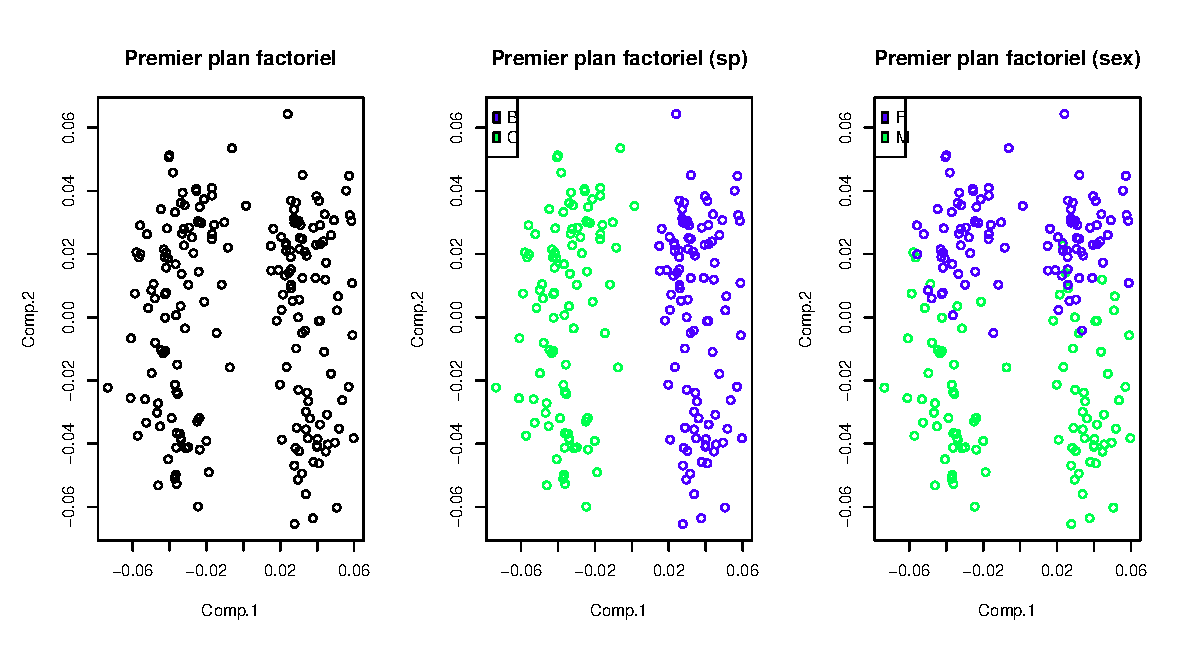
\includegraphics[scale=0.55]{./img/crabs_acp.eps}
\caption{Représentation des données \textit{crabs} par ACP}
\label{crabs_acp}
\end{figure}

On distingue 4 groupes sur la figure de gauche (\ref{crabs_acp}) qui correspondent aux 4 combinaisons d'espèces et de sexe.

La figure du milieu (\ref{crabs_acp}) pour l'espèce montre 2 groupes de données correspondant aux deux espèces de crabes. De même pour la figure de droite (\ref{crabs_acp}) pour le sexe, on remarque qu'il y a un léger recouvrement des données au milieu de cette figure.

Ainsi, on constate bien qu'il y a quatre groupes d'individus différents pour ce jeu de données avec l'ACP.

\subsection*{3.}

Les données Mutations contiennent les mesures de dissimilarités d'une protéine entre différentes espèces.

On effectue l'AFTD sur avec cette mesure de dissimilarités, ici on choisit la représentation à 2 variables (figure \ref{mut_aftd}).

\begin{figure}[H]
\centering
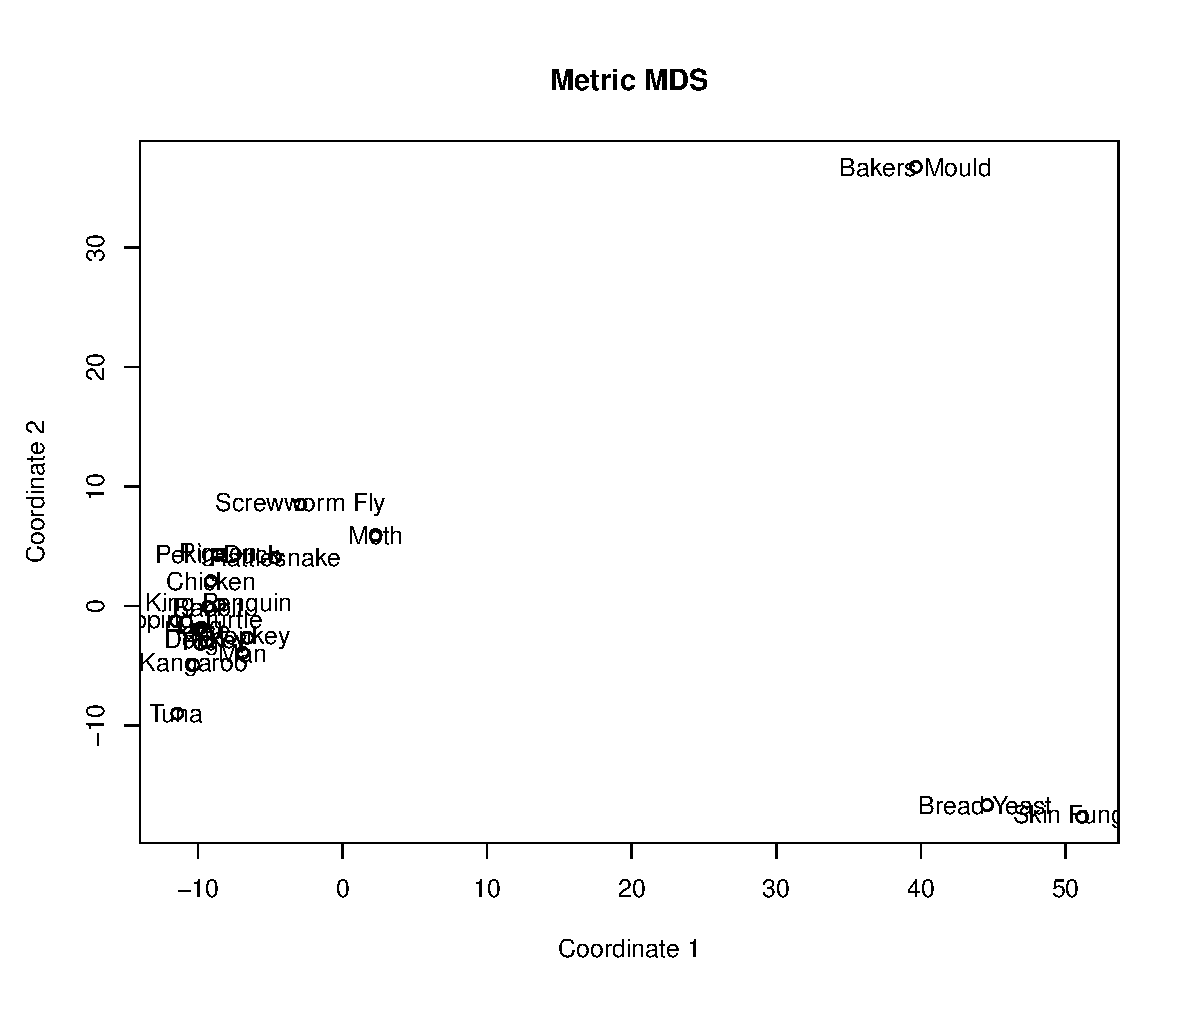
\includegraphics[scale=0.5]{./img/mut_aftd.eps}
\caption{Représentation des données à 2 variables par AFTD}
\label{mut_aftd}
\end{figure}

L'AFTD (\ref{mut_aftd}) montre une grande concentration des points au milieu à droite et des singularités pour $\lbrace Bakers Mould\rbrace$ et $\lbrace Bread Yeast, Skin Fungus\rbrace$.

Pour vérifier la qualité de la représentation, on effectue un diagramme de Shepard qui représente la distance euclidienne en fonction de la dissimilarité. Si la représentation est bonne, les données sont alignées selon la droite $y=x$.

Sur la figure \ref{mut_aftd-comp}, on remarque que plus \textit{d} augmente, plus les données sont alignées selon la bissectrice et donc la qualité de la représentation est meilleure.\\
Pour d=2, la qualité de la représentation est donc moins bonne que pour d=5 par exemple.
\begin{figure}[H]
\centering
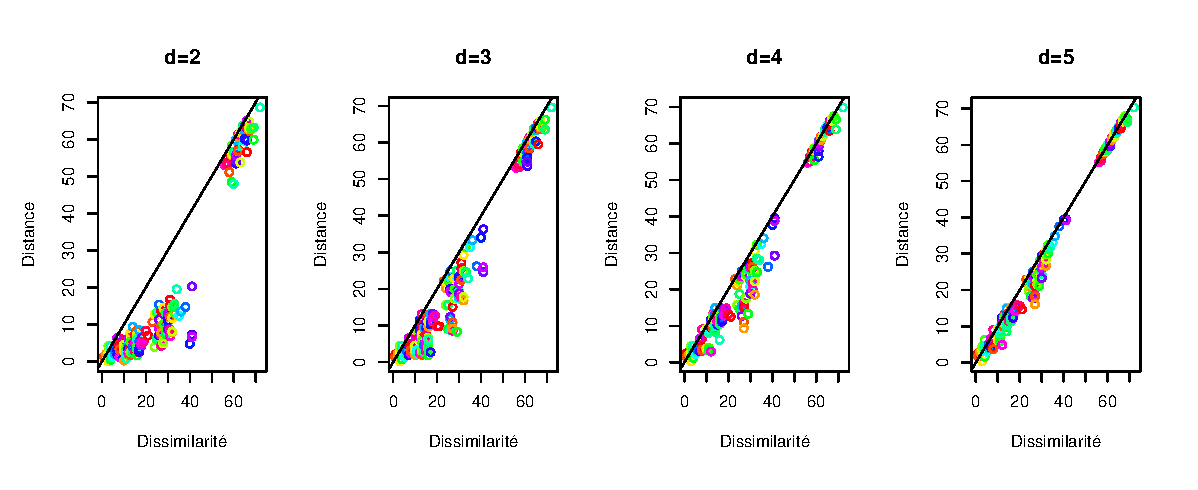
\includegraphics[scale=0.7]{./img/mut_aftd-comp.eps}
\caption{Diagramme de Shepard à \textit{d} variables}
\label{mut_aftd-comp}
\end{figure}


\section{Classification hiérarchique}

Dans cette partie, nous effectuerons des classifications hiérarchiques ascendantes avec la fonction \textit{hclust} et descendantes avec \textit{diana} sur les données \textit{mutations} et \textit{iris}.\\
La classification hiérarchique ne nécessite pas de choisir le nombre de classe à l'avance comparé à l'algorithme des K-Means que l'on étudiera après.
\subsection*{1.}

Nous avons effectué des classifications hiérarchiques ascendantes avec quatre critères d'agrégations différents.\\
La classification hiérarchique ascendante (CAH) part des individus, donc du cas particulier, pour arriver au cas général. (\ref{mut_cah_par})

Les critères d'agrégations utilisés sont les suivants :
\begin{itemize}
\item \textit{complete} : Critère du lien maximum : plus grande distance entre deux classes. $D(A,B)=max\lbrace d(i,i'),i \in A ~ et ~ i'\in B \rbrace$
\item \textit{single} : Critère du lien minimum : plus petite distance entre deux classes. $D(A,B)=min\lbrace d(i,i'),i \in A ~ et ~ i'\in B \rbrace$
\item \textit{ward D2} : Critère de l'inertie intra-classe minimisée au maximum. $D(A,B)=\frac{n_An_B}{n_A+n_B}d^2 (g_a,g_b)$ où $g_i$ est le centre de gravité du sous-espace \textit{i}.
\item \textit{centroid} : Utilise le carré des distances euclidiennes entre les différents centres.
\end{itemize}

Les classifications hiérarchiques obtenues sont très proches de la représentation de l'AFTD. En effet, les différents groupes d'individus de l'AFTD sont bien hiérarchisés distinctement de la même manière.

On remarque que les différents critères d'agrégations groupent l'espèce Bakers Mould avec ou sans Bread Yeast et Skin Fungus, sachant que ces trois espèces sont bien séparées. Les autres individus sont très proches dans la représentation de l'AFTD et sont donc proches dans la hiérarchie.\\
Les méthodes complete et ward D2 ont des résultats similaires et groupent Bakers Mould avec Bread Yeast et Skin Fugus.

Les méthodes single et centroid, séparent l'espèce Bakers Mould et sont donc plus proches de la représentation de l'AFTD.

\begin{figure}[H]
\centering
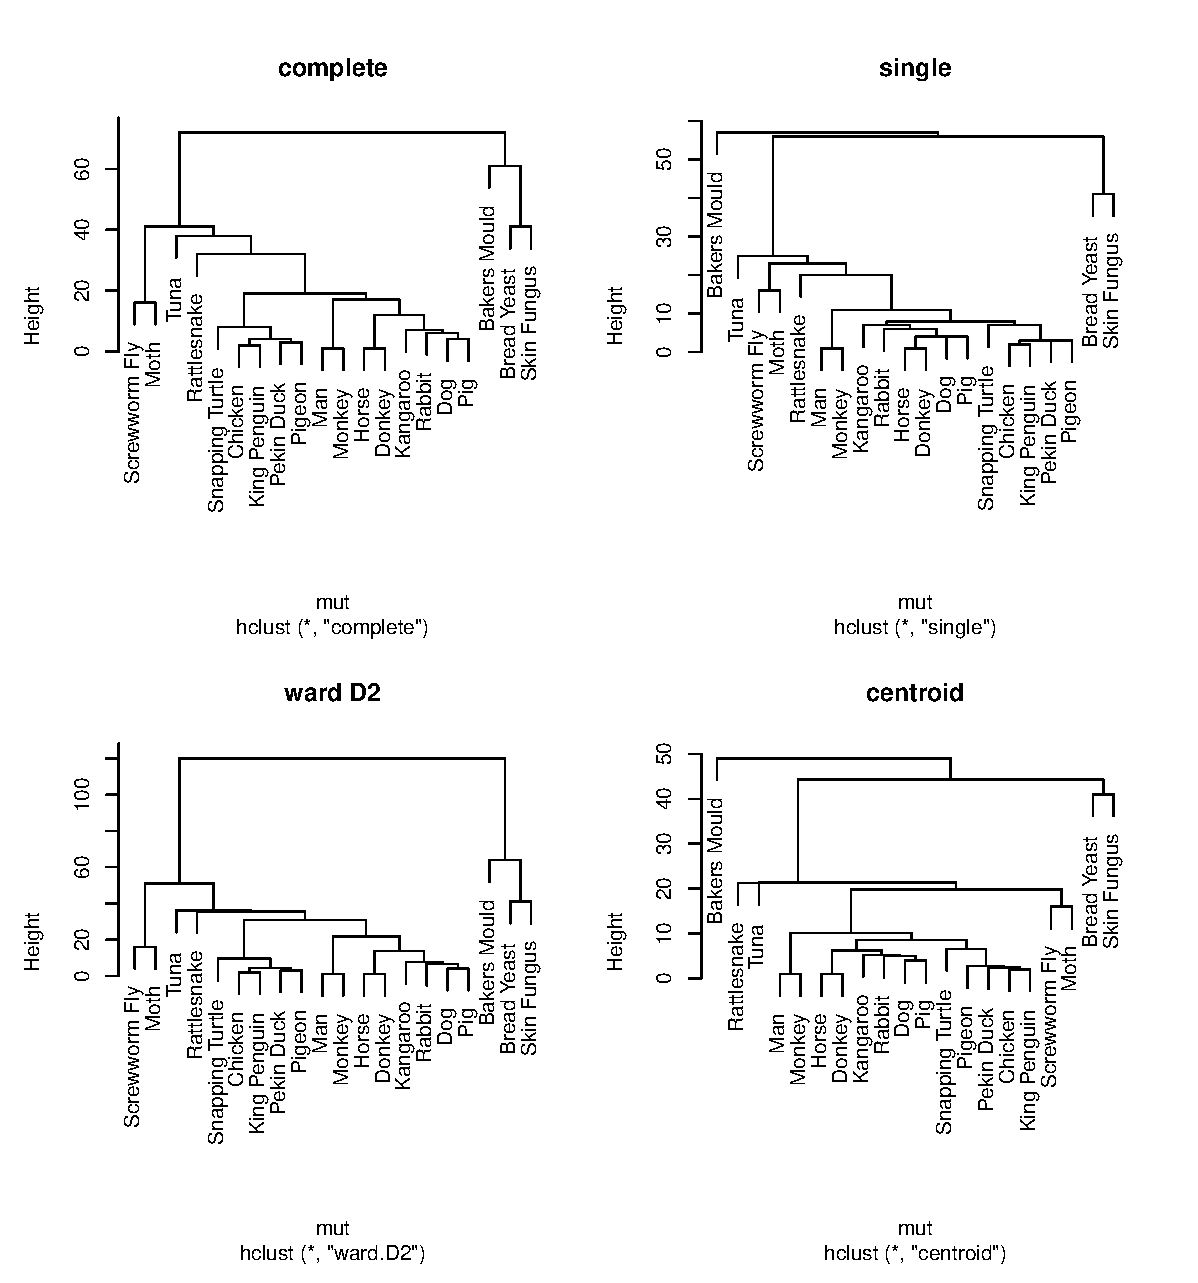
\includegraphics[scale=0.83]{./img/mut_cah_par22.eps}
\caption{Classification hiérarchique ascendante selon différents critères d'aggregations}
\label{mut_cah_par}
\end{figure}


\subsection*{2.}

Avec la classification ascendante hiérarchique (Ward D2) sur Iris (\ref{iris_cah_col}), on obtient 3 groupes hiérarchiques distincts, ce qui correspond bien aux trois espèces d'Iris. De plus, on remarque que la sous hiérarchie à droite groupe les Versicolor et Virginica ensemble, qui sont proches (d'après l'ACP).

\begin{figure}[H]
\centering
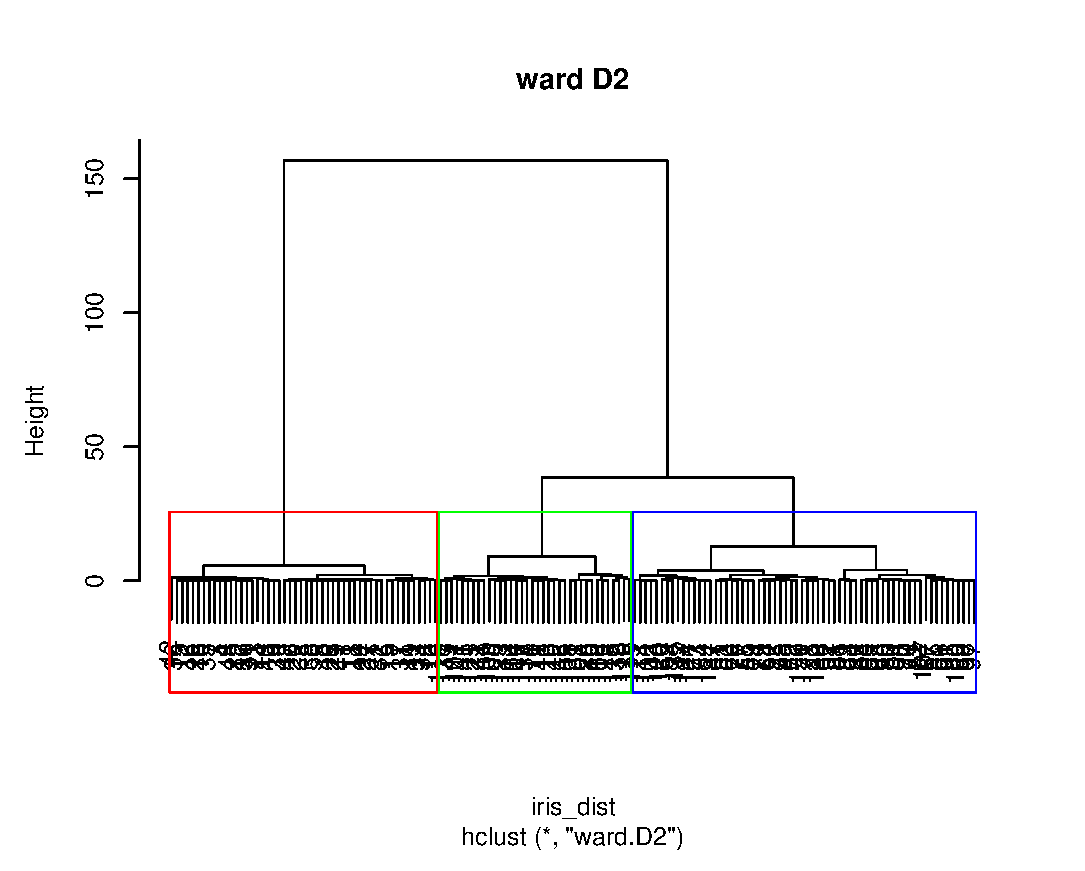
\includegraphics[scale=0.55]{./img/iris_cah_col.eps}
\caption{Classification hiérarchique ascendante}
\label{iris_cah_col}
\end{figure}


\subsection*{3.}

Avec la classification hiérarchique descendante, on part du cas général pour différencier des individus.

La classification est (\ref{iris_cdh}) donc adéquate, car on distingue bien les trois espèces d'Iris. De plus, on remarque que la sous-hiérarchie à droite groupe les Versicolor et Virginica ensemble, qui sont proches (d'après l'ACP).
\begin{figure}[H]
\centering
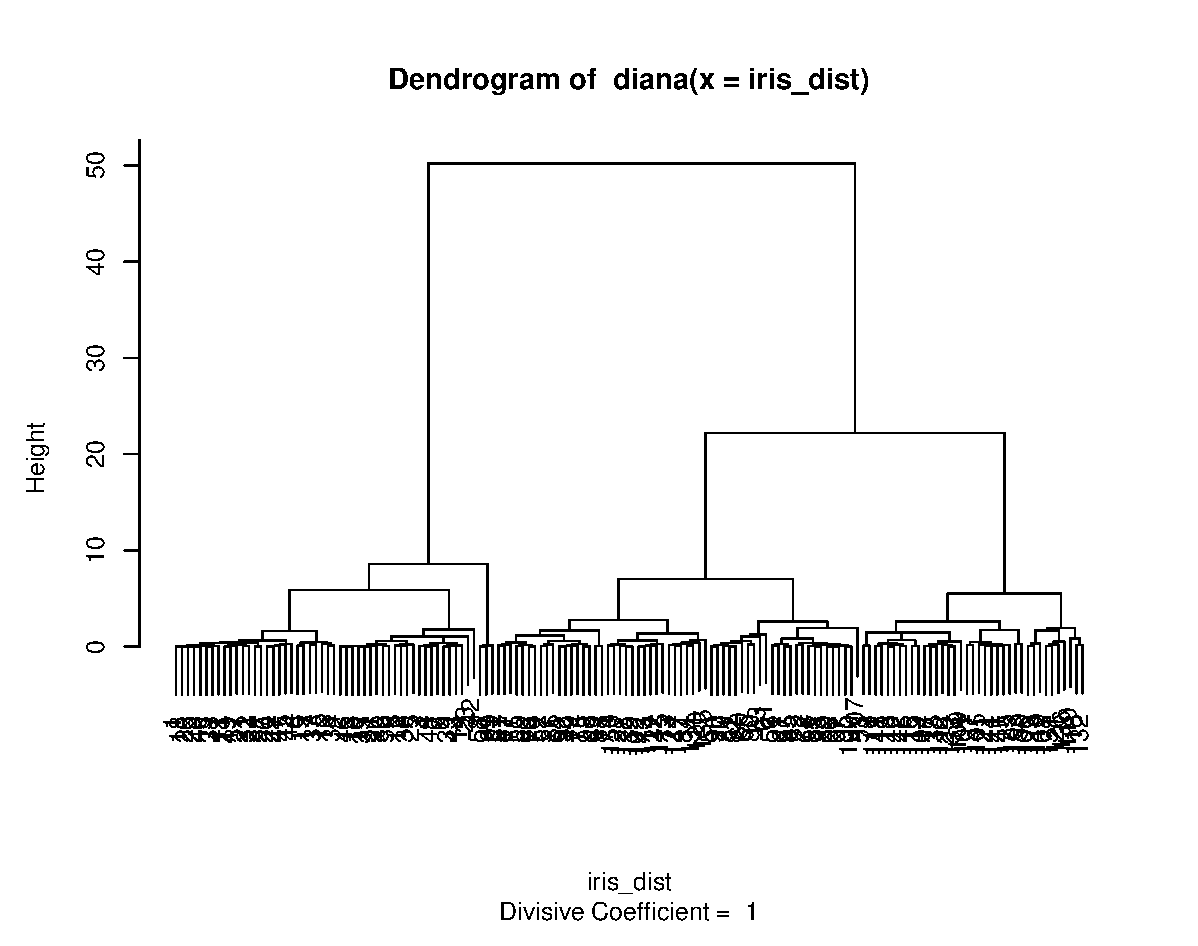
\includegraphics[scale=0.5]{./img/iris_cdh.eps}
\caption{Classification hiérarchique descendante}
\label{iris_cdh}
\end{figure}



\section{Méthodes des centres mobiles}

Dans cette dernière partie, nous appliquerons l'algorithme des K-Means sur les jeux de données précédents pour tenter de trouver le nombre de classes optimales pour classifier les individus.

\subsection{Données Iris}

\subsubsection*{1.}


\begin{figure}[H]
\centering
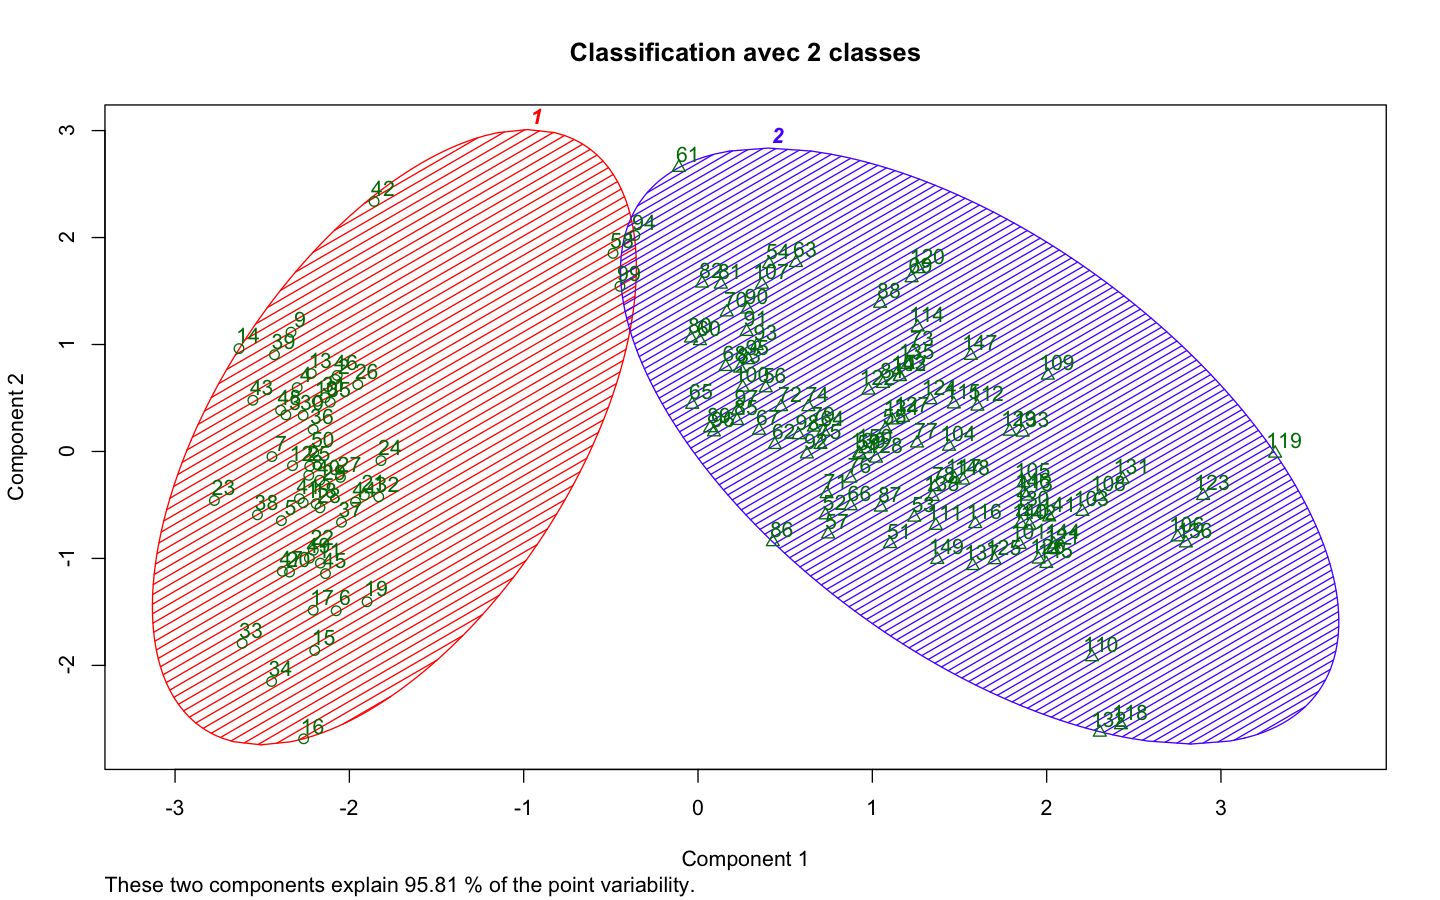
\includegraphics[width=7.5cm]{./img/iris_kmeans_2.png}
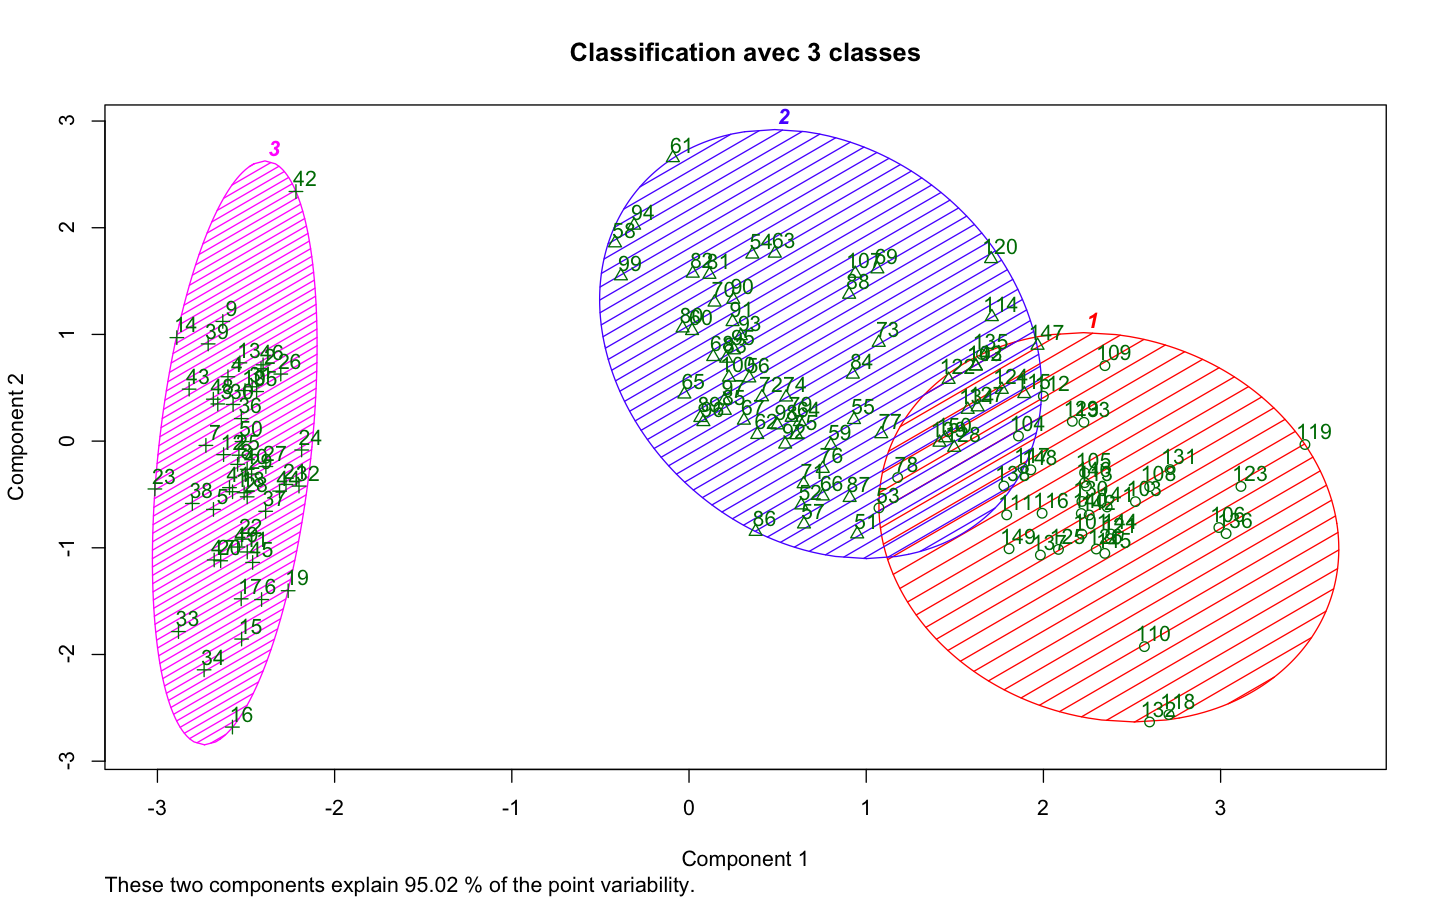
\includegraphics[width=7.5cm]{./img/iris_kmeans_3.png}
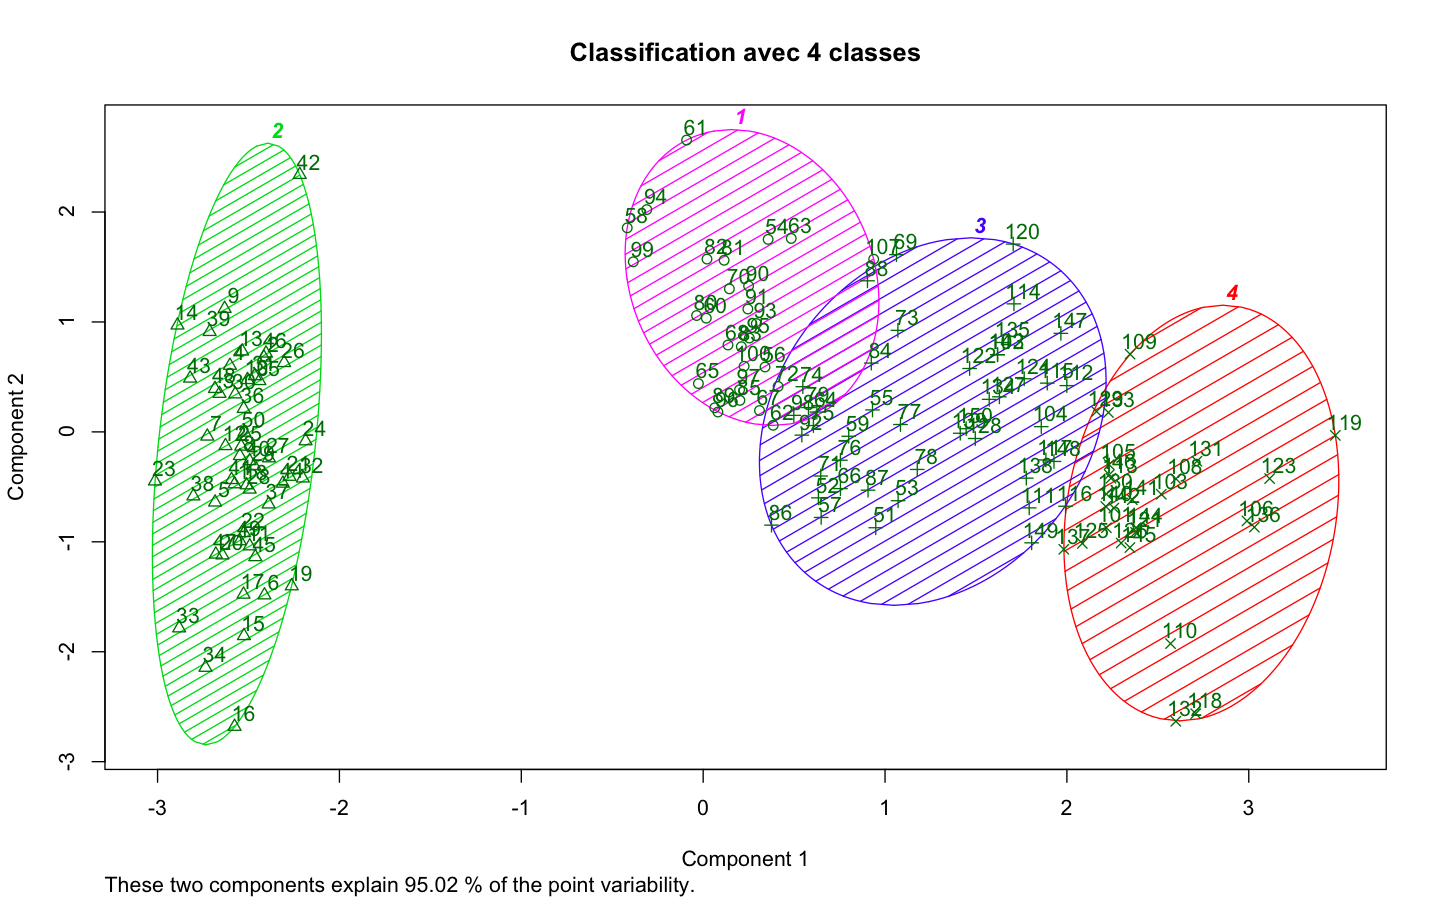
\includegraphics[width=7.5cm]{./img/iris_kmeans_4.png}
\caption{Classification des données iris pour $k \in \lbrack2;4\rbrack$}
\label{iris_kmeans_2_3_4}
\end{figure}

Nous avons appliqué l'algorithme des k-means effectué avec $K \in [2;4]$ (figure \ref{iris_kmeans_2_3_4}).\\
Sachant que le jeu de données a 3 espèces, la partition obtenue pour K=3 classifie bien les individus dans la classe correspondante à l'espèce. Cela vérifie la partition réelle \textit{setosa}, \textit{versicolor}, \textit{virginica}.\\
Pour K=2, k-means fonctionne bien et combine les catégories \textit{versicolor} et \textit{virginica} car ces espèces sont proches, comme nous l'avons vu précédemment.\\
Pour K=4, la classification partitionne les deux espèces de droite (\textit{versicolor}, \textit{virginica}) en 3 catégories.

Il apparaît donc très important de choisir une valeur de K optimale pour l'algorithme des K-Means pour bien interpréter les données et aussi car nous ne sommes pas censés connaître le nombre de classes.


\subsubsection*{2.}
Après avoir effectué plusieurs répétitions de l'algorithme des k-means, on observe que les inerties intra-classes diffèrent et donc les classifications changent aussi.\\



On trouve deux partitions différentes (\ref{iris_kmeans_pour_k_3}). La classification à gauche est une classification optimale plus fréquente que l'autre.\\
L'inertie intra-classe de la classification optimale vaut \textit{78.85}, et l'autre vaut \textit{142.75}.

\begin{figure}[H]
\centering
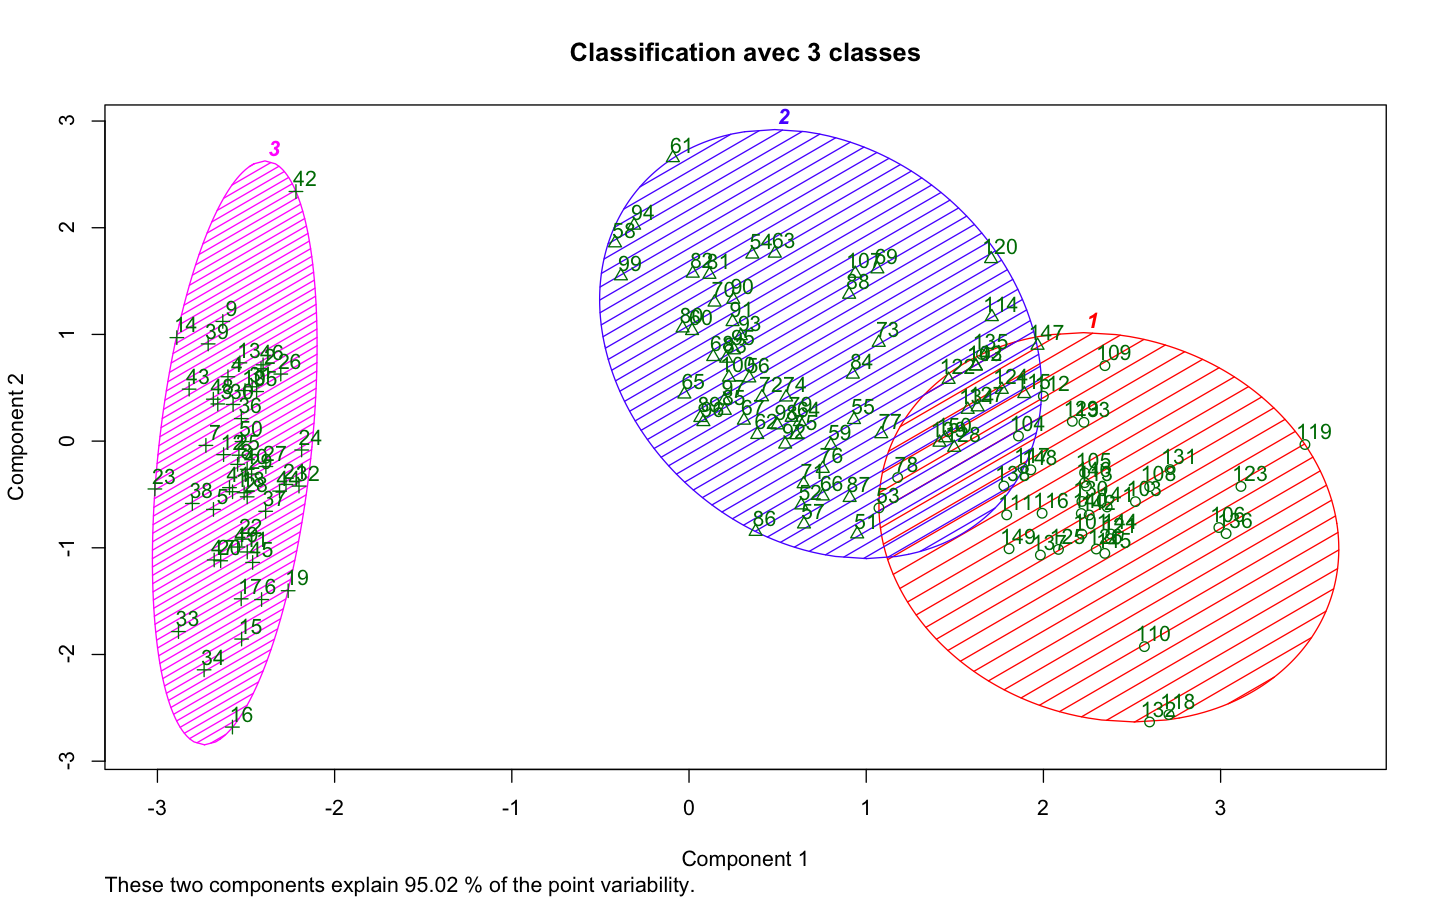
\includegraphics[width=7.5cm]{./img/iris_kmeans_3.png}
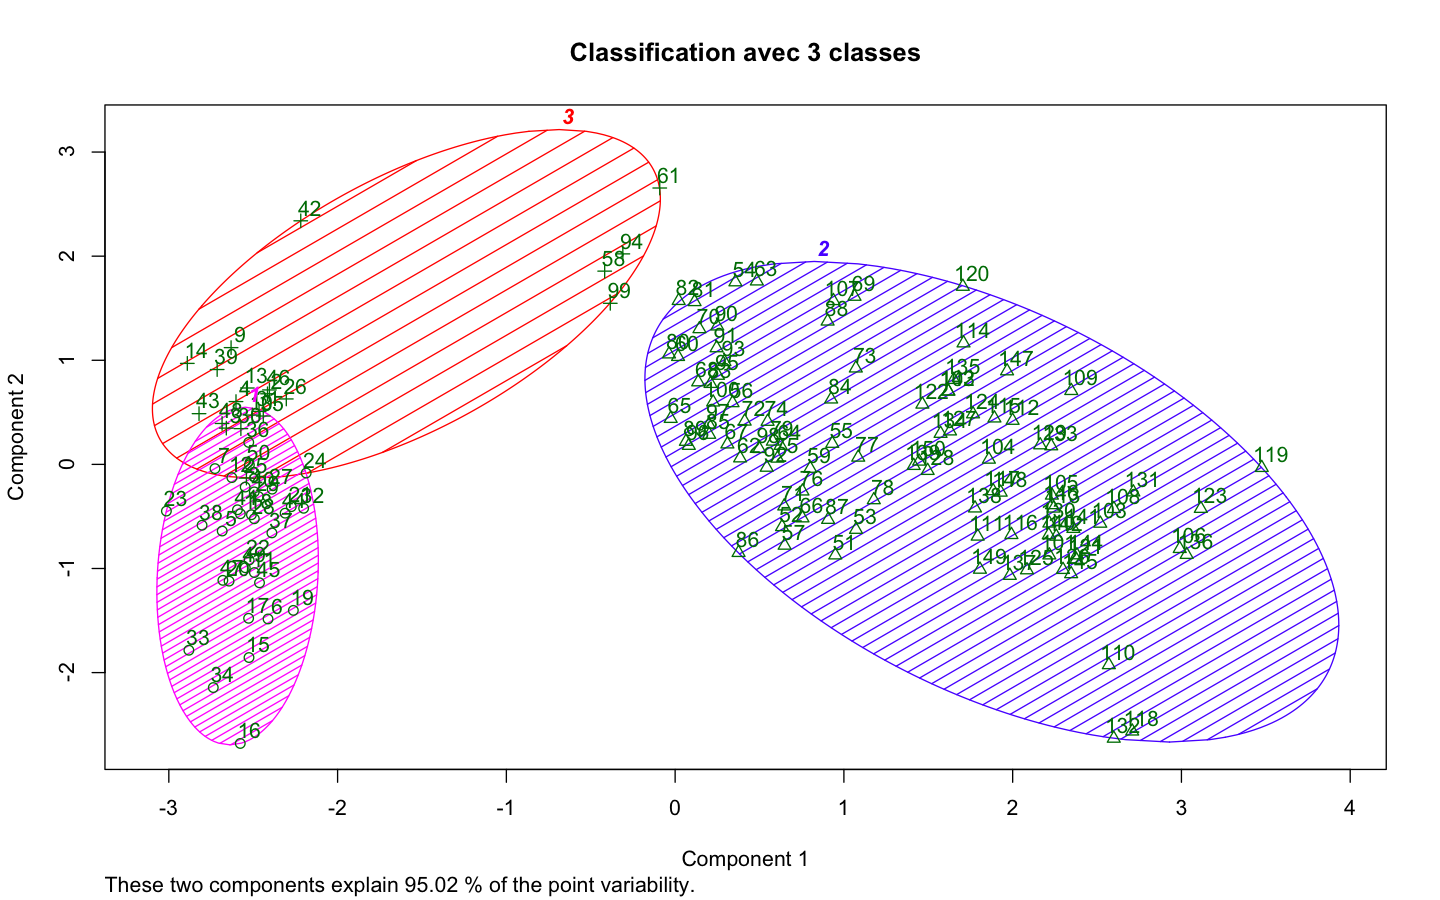
\includegraphics[width=7.5cm]{./img/iris_kmeans_3_2.png}
\caption{Classification des données iris pour k=3}
\label{iris_kmeans_pour_k_3}
\end{figure}

Cette variation dans le résultat est due à la sélection aléatoire des points initiaux des centres au début de l'algorithme, qui nous donne un minimum local et pas forcément un minimum global.

\subsubsection*{3.}\label{3.1.3}
Après avoir effectué 100 répétitions de l'algorithme des K-means, pour $K \in [1;10]$, on trace l'inertie intra-classe minimale en fonction de K sur les 100 répétitions (figure \ref{iris_inertie_min}).\\

\begin{figure}[H]
\centering
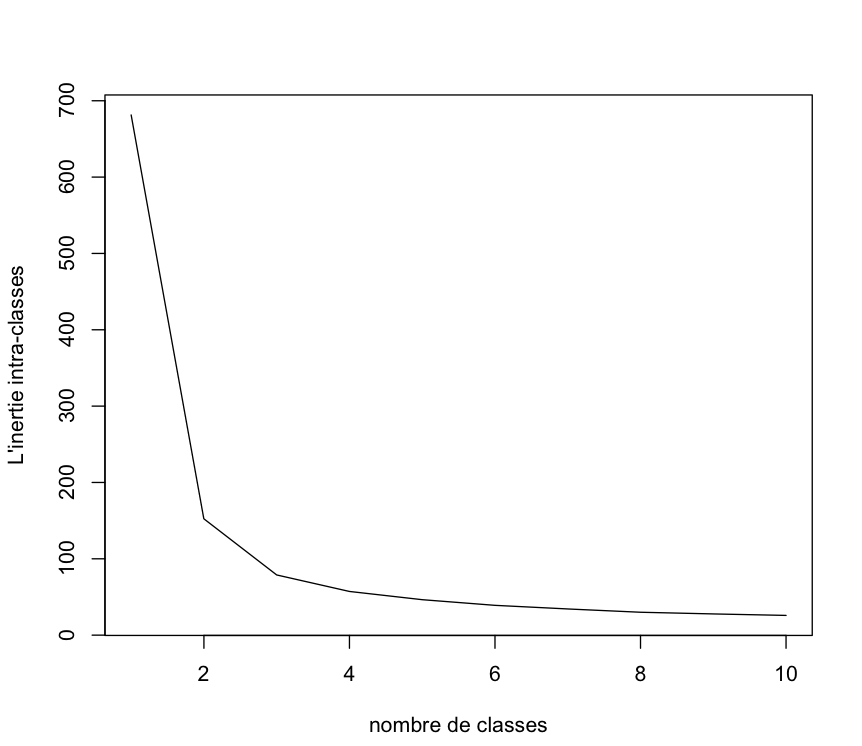
\includegraphics[scale=0.235]{./img/iris_inertie_min.png}
\caption{Inertie minimale en fonction de K}
\label{iris_inertie_min}
\end{figure}

D'après la méthode du coude, on trouve qu'une partition à K=2 ou K=3 classes est possible. On propose donc de classifier ce jeu de données par 3 classes, car celle-ci possède une classification avec une inertie intra-classe assez faible.\\
Pour un nombre de classes égal ou plus grand que 3, l'inertie est un peu plus faible, mais pas de beaucoup donc ces partitions ne sont pas intéressantes.

\subsubsection*{4.}

\begin{figure}[H]
\centering
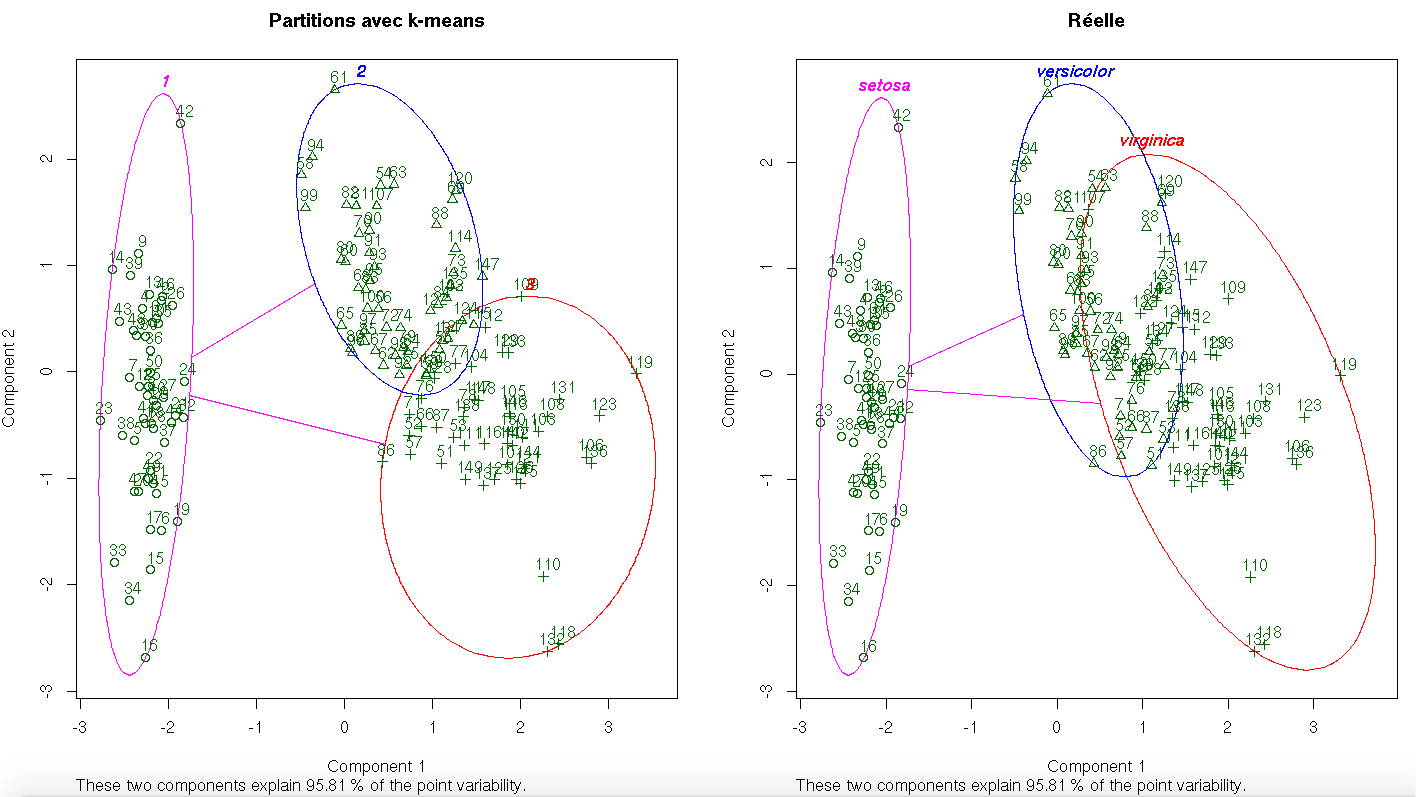
\includegraphics[width=13cm]{./img/iris_classification_reelle.png}
\caption{Comparaison du résultat de k-means et la partition réelle}
\label{iris_classification_reelle}
\end{figure}

On peut observer que la partition obtenue par les centres mobiles et la partition réelle sont similaires sur la figure \ref{iris_classification_reelle}, à condition que l'on choisisse bien la valeur de K.\\
La groupe 1 obtenu par k-means est bien identifié par l'espèce \textit{setosa}, mais les groupes 2 et 3 se recouvrent un peu.\\
Le résultat est donc satisfaisant.

\subsection{Données Crabs}

\subsubsection*{1.}

\begin{figure}[H]
\centering
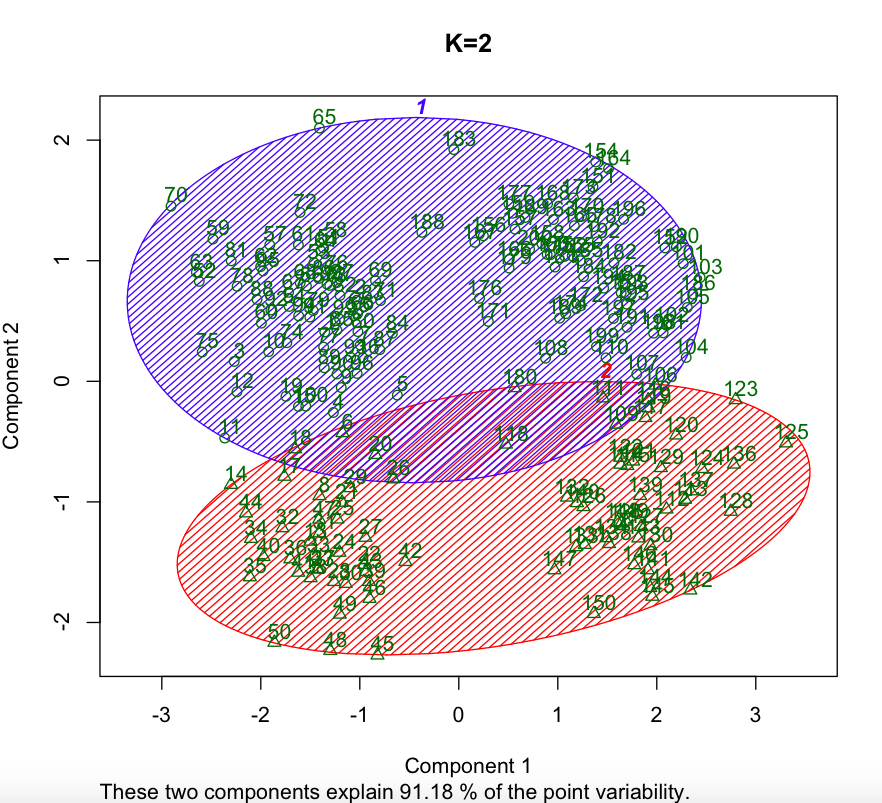
\includegraphics[width=7cm]{./img/crabs_kmeans_2.png}
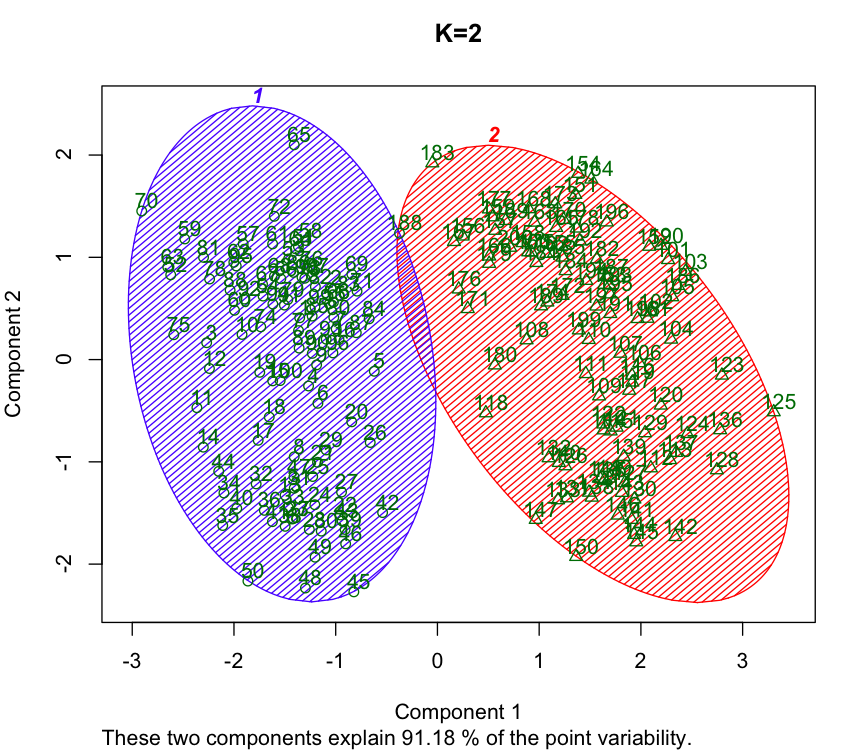
\includegraphics[width=7.2cm]{./img/crabs_kmeans_2_2.png}
\caption{Classification de crabs par k-means avec 2 classes}
\label{crabs_kmeans_2}
\end{figure}

Les résultats obtenus ne sont pas toujours les mêmes. On trouve 2 différentes partitions. Autrement dit, il existe 2 valeurs minimales locales pour l'inertie intra-classes.\\ 
D'après la figure de l'exercice précédent (figure \ref{crabs_acp}), on en déduit que la classification à gauche correspond à la classification du sexe et la classification à droite correspond à l'espèce.


\subsubsection*{2.}

On applique maintenant l'algorithme des K-Means avec K=4

\begin{figure}[H]
\centering
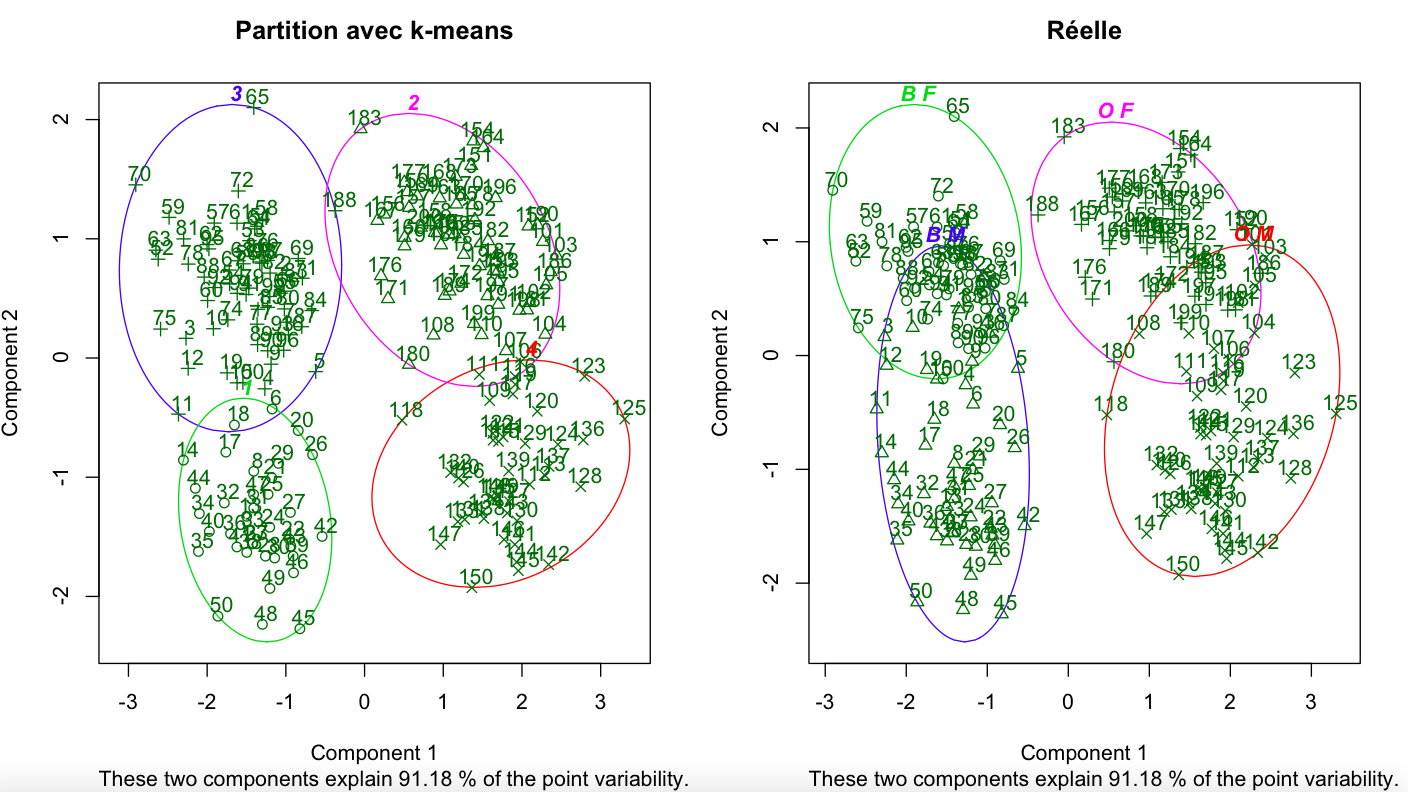
\includegraphics[width=13cm]{./img/crabs_classification_reelle.png}
\caption{La classification par k-means et la partition réelle}
\label{crabs_comparaison}
\end{figure}

L'étude des 2 graphiques \ref{crabs_comparaison} nous montre que la partition obtenue par les k-means correspond bien à la partition réelle si l'on choisit la bonne valeur pour K. Il y a des erreurs de classification due à la similarité de certains individus et du chevauchement dans la classification réelle. Globalement, la classification est similaire à la partition réelle.


\subsection{Données Mutations}

\subsubsection*{1.}

On applique l'algorithme des K-Means sur le jeu de données Mutations en cherchant si différentes classifications existent pour K=3.

\begin{figure}[H]
\centering
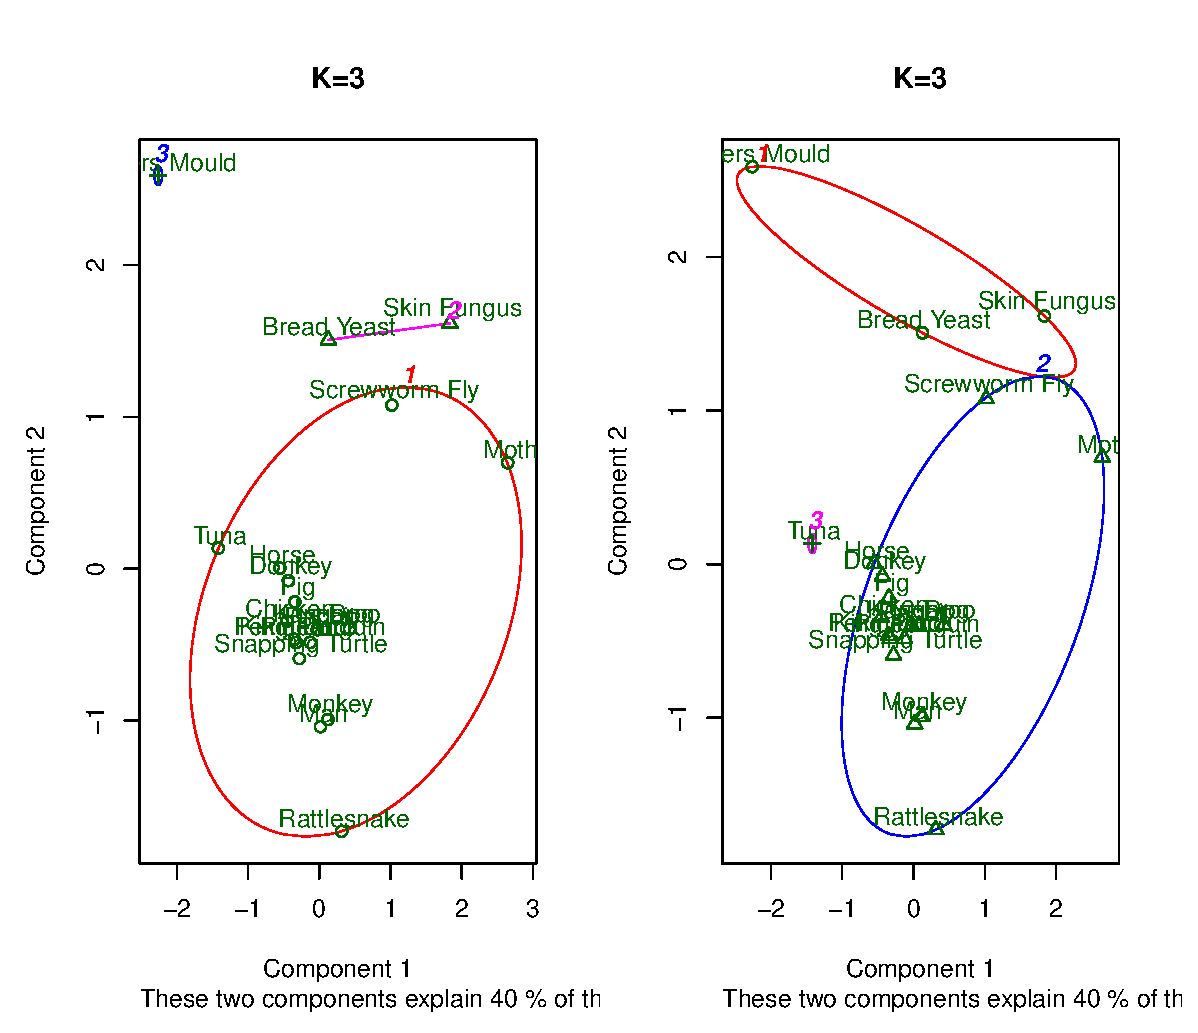
\includegraphics[scale=0.5]{./img/mut_clusplot_aftd_comp.eps}
\caption{Classifications à 3 classes avec K-Means}
\label{mut_clusplot_aftd-comp}
\end{figure}

Nous avons donc trouvé deux classifications différentes (\ref{mut_clusplot_aftd-comp}).

\subsubsection*{2.}

Pour étudier la stabilité des classifications trouvées, on calcule la variance pour chaque \textit{K} variant de 2 à 5 (table \ref{tab3.3.2_var}). La variance la plus faible correspond à la partition \textit{K} la plus stable.

On représente d'abord l'inertie intra-classe en fonction de K de la même manière qu'en [\ref{3.1.3}].

La figure \ref{mut_elbow} montre clairement que la partition optimale par la méthode du coude est pour K=2.
\begin{figure}[H]
\centering
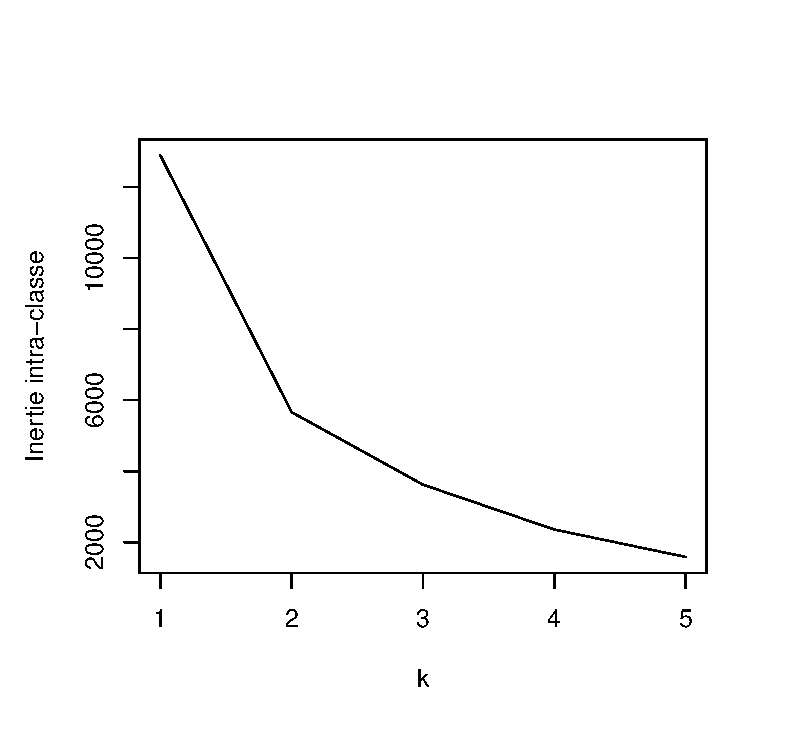
\includegraphics[width=5.7cm]{./img/mut_elbow.eps}
\caption{Inertie intra-classe en fonction de K}
\label{mut_elbow}
\end{figure}

% \begin{table}[H]
% \caption{Inertie intra-classe pour différents \textit{k}}\label{tab3.3.2}
% \centering
% \begin{tabular}{l|cccc}
% k& k=2 & k=3 & k=4 & k=5 \\
% \hline
% Inertie intra-classe & 5660 & 3622 & 2360 & 1590 
% \end{tabular}
% \end{table}

En calculant la variance des inerties intra-classe pour chaque K, on remarque qu'elle est nulle pour K=2, donc cette partition est parfaitement stable.

On choisit donc d'appliquer un K-Means avec K=2 sur les données mutations (\ref{mut_clusplot_k2}).

\begin{figure}[H]
\centering
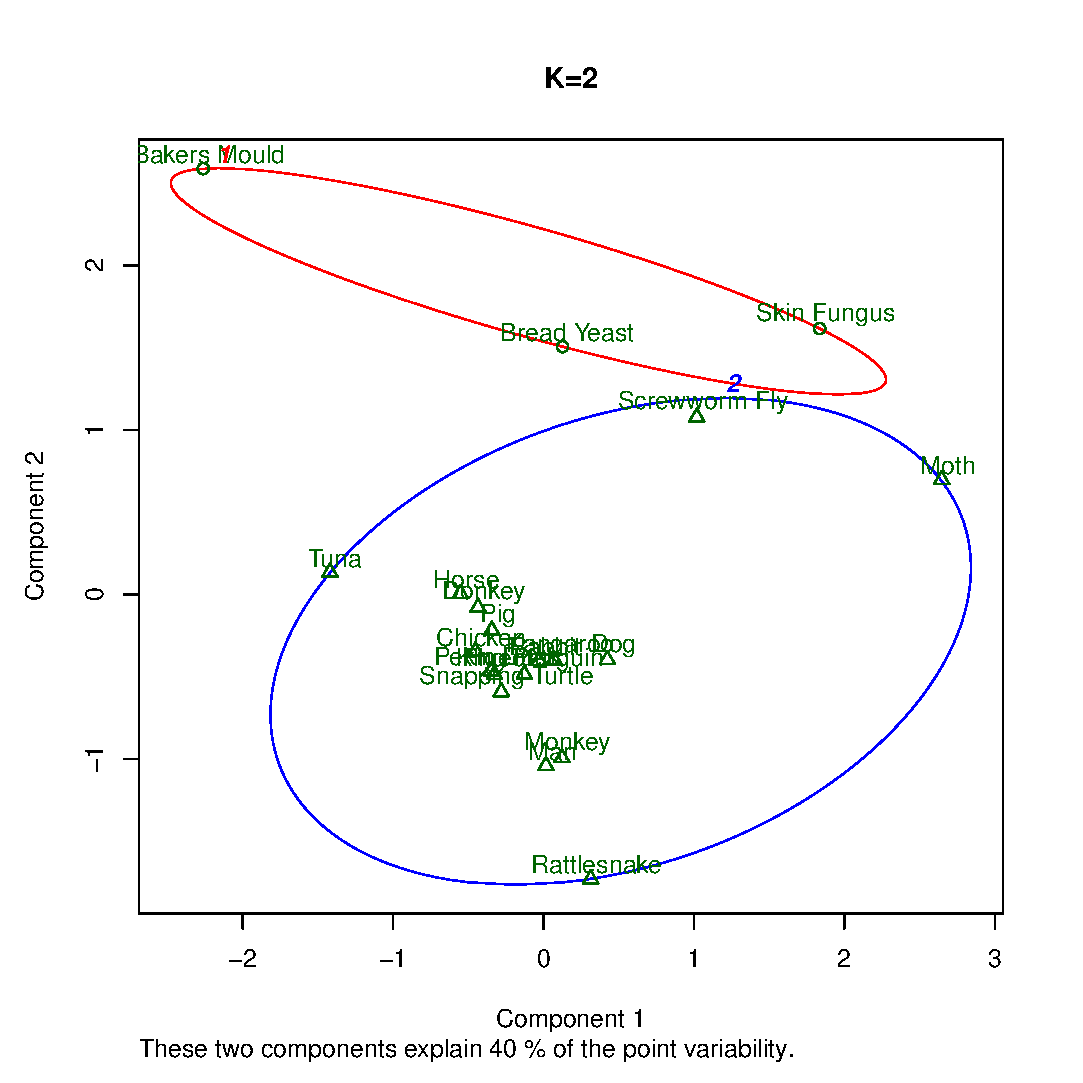
\includegraphics[scale=0.48]{./img/mut_clusplot_k2.eps}
\caption{Classifications à 2 classes avec K-Means}
\label{mut_clusplot_k2}
\end{figure}












\section*{Conclusion}
%%%% TO DO
Ce TP nous a permis d'appliquer différents algorithmes de classification automatique afin de chercher à regrouper des données ensemble. Nous avons cherché à trouver le nombre de classifications optimales, qui représente le mieux les données.\\
La visualisation des données nous a aussi été utile pour avoir une première intuition sur nos données et leurs groupements possibles. De plus, cela nous a aidés à choisir un nombre de partitions finales.

La classification automatique permet donc d'aborder les problèmes de l'apprentissage non supervisé en identifiant des patterns dans les données.


%\begin{thebibliography}{99} 
\section*{Références}
[1] \href{https://stat.ethz.ch/R-manual/R-devel/library/stats/html/hclust.html}{Hierarchical Clustering}

[2] \href{https://stat.ethz.ch/R-manual/R-devel/library/stats/html/kmeans.html}{K-Means Clustering}

[3] \href{http://www.statmethods.net/advstats/cluster.html}{Quick-R: Cluster analysis}

%\bibitem [1]{stock} \href{http://www.sthda.com/english/wiki/principal-component-analysis-in-r-prcomp-vs-princomp-r-software-and-data-mining}{Principal component analysis in R : prcomp() vs. princomp() - R software and data mining}


\section*{Annexes}

% à mettre en annexe
\begin{table}[H]
\caption{Variance des inerties intra-classe pour différents \textit{k}}\label{tab3.3.2_var}
\centering
\begin{tabular}{l|cccc}
k & k=2 & k=3 & k=4 & k=5 \\
\hline
Variance & 0 & 365494 &537365 &468997
\end{tabular}
\end{table}


%\end{thebibliography}


%----------------------------------------------------------------------------------------
%\end{multicols}
\end{document}
